\documentclass[11pt, letterpaper]{report}
%basic packages
\usepackage[utf8]{inputenc}
\usepackage[T1]{fontenc}
\usepackage{graphicx}
\usepackage[margin=1in]{geometry}
\usepackage[usenames,dvipsnames]{xcolor}

%math
\usepackage{amsmath, amsthm, amsfonts, amssymb, mathtools}
\usepackage{mathrsfs}
\usepackage{cancel}
\usepackage{siunitx} %phyjsicsssss
\usepackage{bbm} %mathbb for numbers
\usepackage[all]{xy} % https://texdoc.org/serve/xyguide.pdf/0
\makeatletter
\renewcommand*\env@matrix[1][c]{\hskip -\arraycolsep
  \let\@ifnextchar\new@ifnextchar
  \array{*\c@MaxMatrixCols #1}}
\makeatother %matrix realignment

%misc
\usepackage{float}
\usepackage[hyphens]{url}
%\definecolor{page}{HTML}{242526}
%\pagecolor{page}
\usepackage{booktabs} %the \toprule and \bottomrule thick lines on tables
\usepackage{hyperref}

%my commands
\DeclarePairedDelimiter\bra{\langle}{\rvert} %Bra
\DeclarePairedDelimiter\ket{\lvert}{\rangle} %Ket
\DeclarePairedDelimiterX\braket[2]{\langle}{\rangle}{#1\,\delimsize\vert\,\mathopen{}#2} %Bra-ket
\newcommand{\pvec}[1]{\vec{#1}\mkern2mu\vphantom{#1}} % from https://tex.stackexchange.com/questions/120029/how-to-typeset-a-primed-vector
\newcommand{\hati}{\boldsymbol{\hat{\textbf{\i}}}}
\newcommand{\hatj}{\boldsymbol{\hat{\textbf{\j}}}}
\newcommand{\hatk}{\boldsymbol{\hat{\textbf{k}}}}
\newcommand{\R}{\mathbb{R}}
\DeclareMathOperator{\diag}{diag}
\DeclareMathOperator*{\argmax}{arg\,max}
\DeclareMathOperator*{\argmin}{arg\,min}

%theorems
\usepackage{tikz}
\usepackage{tikz-cd}
\usepackage[framemethod=TikZ]{mdframed}
\usepackage{thmtools}
\newtheorem{theorem}{Theorem}
\newtheorem{corollary}{Corollary}
\newtheorem{lemma}{Lemma}
\newtheorem{proposition}{Proposition}

% slightly neater (imo) theorems
%\declaretheoremstyle[headfont=\bfseries, bodyfont=\normalfont, mdframed={linewidth=1pt, bottomline=false, topline=false, rightline=false, leftline=false}]{theorem}
%\declaretheorem[numbered=yes, style=theorem, name=Theorem]{theorem}
%\declaretheorem[numbered=yes, style=theorem, name=Lemma]{lemma}
%\declaretheorem[numbered=yes, style=theorem, name=Corollary]{corollary}
%\declaretheorem[numbered=yes, style=theorem, name=Proposition]{proposition}

% Side Indented Theorems - https://tex.stackexchange.com/questions/429339/shifting-newtheorem
\newtheoremstyle{side}{}{}{\advance\leftskip3cm\relax\itshape\normalfont}{-4pt}
{\bfseries}{}{0pt}{
\makebox[0pt][r]{
  \smash{\parbox[t]{2.5cm}{\raggedright\thmname{#1}.
  \thmnote{\newline(#3)}}}
  \hspace{10.1pt}}}

\theoremstyle{side}
\newtheorem*{note}{Note}
\newtheorem*{intuition}{Intuition}
\newtheorem*{claim}{Claim}
\newtheorem*{prev}{As Previously Seen}

\theoremstyle{definition}
\newtheorem{definition}{Definition}
\newtheorem*{remark}{Remark}
\newtheorem*{example}{Example}
\newtheorem*{notation}{Notation}

\renewcommand{\qedsymbol}{$\blacksquare$}
\declaretheoremstyle[headfont=\bfseries, bodyfont=\normalfont, mdframed={linewidth=1pt, bottomline=false, topline=false, rightline=false, innertopmargin=0pt, innerbottommargin=0pt}, qed=\qedsymbol]{proof}
\declaretheorem[numbered=no, style=proof, name=Proof]{replacementproof}
\renewenvironment{proof}[1][]{\begin{replacementproof}}{\end{replacementproof}}

%fancy headers
\usepackage{fancyhdr}
\pagestyle{fancy}
\fancyhead{}\fancyfoot{}
\fancyfoot[R]{\thepage}
\fancyfoot[C]{\leftmark}

%lectures, taken from (https://castel.dev/post/lecture-notes-3)
\makeatother
\def\@lecture{}%
\newcommand{\lecture}[3]{%
	\ifthenelse{\isempty{#3}}{%

		\def\@lecture{Lecture #1}%
	}{%
		\def\@lecture{Lecture #1: #3}
	}
	\subsection*{\@lecture}
	\hfill{\small\textsf{#2}}\par
}
\makeatletter
\author{Grant Talbert}

\title{General Physics 2: Lab 1 Report}
\date{09/20/24}
\renewcommand{\thesection}{\arabic{section}}
\usepackage{pgfplots}
\hypersetup{
    colorlinks,
    linkcolor={black},
    urlcolor={black},
    citecolor={black}
}
\begin{document}
\maketitle
\begin{abstract}
	This paper attempts to verify the relationship $F\propto  r^{-2}$ present in Coulomb's law via experimental data. We find that the power of $r$ is $-1.04$, and we observe an error of $\pm0.47$. Since our experimental values do not agree with the theoretical values within the given error, we assume there was either an error in the setup, or charge leakage had a significant impact on the data.
\end{abstract}
\section{Theory}
Coulomb's law stats that for two point charges with magnitudes $q_1$ and $q_2$, the force from charge 1 on charge 2 $\mathbf{F}_{12}$ is
\[
	\mathbf{F}_{12}=k_e \frac{q_1q_2}{r^2}\mathbf{\hat{r}}
.\]
In this case, $\mathbf{\hat{r}}$ is a unit vector pointing in the direction of the force. From this, it follows that the magnitude of the forces between the two charges is
\[
	F=k_e \frac{q_1q_2}{r^2}
.\]
The purpose of this lab is to verify that $F$ is indeed proportional to $r^{-2}$.

Unfortunately, we do not have access to point charges, so we used charged spheres. Maintaining the accuracy of the result requires a correction factor $B$, given as
\[
	B=1-4\left( \frac{a^3}{r^3} \right) \]
for sphere radius $a$ and distance $r$. This correction factor will be discussed more in the section on error analysis.

Due to Coulomb's law, if we hold two point charges near each other, they should exert a nonzero force on each other, the magnitude of which we can measure. Since the purpose of this force is to verify the relationship between $F$ and $r$, we will take measurements of $F$ for varying values of $r$, and attempt to measure a slope.

The method of measuring force involves measuring torque, which has a magnitude $\tau =K\theta $ for some twist constant $K$. Since $\tau =Fd$ for $d$ being the distance from the point of rotation that the force $F$ is applied at, we have
\[
	F=\frac{\tau}{r}=\frac{K\theta }{d}
.\]
Since the goal of this experiment is only to prove the inverse proportionality relationship of $F$ and $r^2$, we can ignore the twist constant $K$ in our analysis.

If we have $F$ being the electric force between two charges, then we can take
\[
	F=ar^n
\]
for some unknown constant $a$, and thus the goal of the experiment is to show $n=-2$. It follows that we have
\[
	ar^n=\frac{K\theta }{d}
,\]
and thus,
\[
	\theta =r^n \frac{ad}{K}
.\]
We can absorb our coefficients $ad/K$ into one coefficient, which we call $b$. Thus,
 \[
	\theta =br^n
.\]
Since $\ln \theta =n\ln r+\ln b$, we have the slope of the graph of $\ln \theta $ vs $\ln r$ is just $n$. This calculation does not depend on other constants, and allows us to verify the relationship between $F$ and $r$. In our analysis, we will find a value of $n$ based on experimental data in this manner.
\section{Procedures}
The experimental apparatus involves two identical charged spheres held at an identical height. One charged sphere was fixed in place, and the other charged sphere was held on the end of a rod attached to a thin metal wire, allowing it to rotate. The force between the spheres would exert a force on the two balls. Since the ball attached to a rod was capable of rotating, it would move subject to this force. The wire exerts a torque in the opposite direction as it is turned more, leading to some equilibrium point wherein the torque from the wire matched the torque from the electric force.

The wire can be manually rotated by some angle $\theta $, which we can record. This rotation applies increased torque on the system, allowing us to modify the equilibrium point. By having the equilibrium point be the same spatial position while letting the distance between the balls $r$ vary, we are able to see how the force varies by seeing how the $\theta $ required to maintain the equilibrium position varies. We can then slide the fixed ball to vary $r$. The rotating ball has a marker that lines up with a stationary marker when it is oriented in the correct direction, such that the Coulomb force $F$ is perpendicular to the rod it is attached to. We choose this to be the position we want the sphere's equilibrium position to be to maximize the torque due to the force, making the analysis much easier.
\begin{center}
	\begin{figure}[ht]
	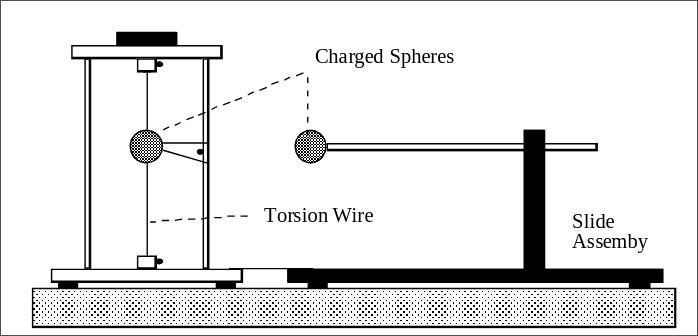
\includegraphics[scale=0.5]{../figures/experiment.png}
	\centering
	\caption{Experimental Apparatus}\label{fig:1}
\end{figure}
\end{center}

Charge can naturally leak due to random variables such as humidity, so to ensure the accuracy of our measurements, we took three measurements for each given $r$, and we measured many values of $r$. Additionally, we used a ground to discharge and a charging probe to recharge the spheres between every measurement, to prevent charge leakage from having a significant long-term impact.

Taking everything into account, we have the following list of procedures.
\begin{enumerate}
	\item Discharge the spheres with the grounded probe. Move the sliding sphere as far away as possible.
	\item Using a charging probe, charge both spheres with 5000V of energy. Take proper saftey precautions while handling high voltage energy and turn it off after charging.
	\item Slide the sliding sphere until the distance between the centers of the two spheres (marked on the bottom of the slider) is $r=20\text{cm}$.
	\item Adjust the torsion knob until the markers line up for the rotating sphere. Read and record the $\theta $ on the torsion knob.
	\item Repeat steps 1 through 4 three times for each value of $r$. Record data for $r$ values of 20cm, 15cm, 12cm, 10cm, 8cm, 7cm, 6cm, and 5cm.
\end{enumerate}
\section{Data and Error Analysis}
Our torsion knob read $\theta =330^\circ $ when no force was exerted, so to normalize our values of $\theta $, we subtracted $330^\circ $ from each measurement. For example, if we measured $340^\circ $, we would record $\theta =340^\circ -330^\circ =10^\circ $. Our data is recorded in \hyperref[tab:1]{table 1}. Since we measured 3 $\theta $ values, we denoted the first trial values as $\theta _1$, the second trial as $\theta _2$, and the third trial as $\theta _3$. This table also includes the averages of $\theta $ for each value of $r$, denoted $\overline{\theta } $.
\begin{center}
	Table 1: Measurements of $\theta $.\\\vspace*{5pt}\label{tab:1}
	\begin{tabular}{c|c|c|c|c}
		$r$ (cm)&$\theta_1$ (degrees)&$\theta_2$ (degrees)&$\theta_3$ (degrees)&$\overline{\theta } $ (degrees)\\
		\hline
		20&14&20&20&18\\
		15&22&28&28&26\\
		12&39&39&39&39\\
		10&45&45&45&45\\
		8&64&51&51&55\\
		7&70&70&70&70\\
		6&80&76&80&79\\
		5&101&101&101&101
	\end{tabular}
\end{center}

Since we are not using point charges, but conducting spheres, there is some error present in the distribution of the charges within the sphere. The force they exert as they approach pushes charges away, modifying the force from that of a point charge. If we take $a$ to be the radius of the sphere, then it has been given that the method to correct for this is to divide each value of $\theta $ by the factor
 \[
	B=1-4\left( \frac{a^3}{r^3} \right) 
.\]
Each sphere has a diameter of 4cm, and thus a radius of 2cm, so we have
\[
	B=1-4\left( \frac{8}{r^3} \right) 
.\]
For example, in the case of $r=8 $cm, we have
\[
	B=1-4\left( \frac{8}{8^3} \right) =1-\frac{4}{64}=\frac{60}{64}=\frac{15}{16}
.\]
Dividing our $\theta_1$ value of $64^\circ $ by this gives the corrected value $\theta_1'$ of
\[
	\theta_1' = 64\cdot \frac{15}{16}=4\cdot 15=60
.\]
\hyperref[tab:2]{Table 2} depicts the corrected values of $\theta $. We only need to apply this correcting value to the average, since it's just a multiple and can factor out, so this table only depicts the corrected averages, denoted $\theta '$.

\begin{center}
	Table 2: Corrected values of $\theta $.\label{tab:1}\\\vspace*{5pt}
	\begin{tabular}{c|c}
		$r$ (cm)&$\theta '$ (degrees)\\
		\hline
		20&18\\
		15&26\\
		12&38\\
		10&44\\
		8&52\\
		7&63\\
		6&67\\
		5&75
	\end{tabular}
\end{center}

As outlined in the section on theory, we need to find $\ln r$ and $\ln \theta'$. Recall that, for $F\propto r^n$,
\[
	\ln \theta '=n\ln r+\ln b
\]
for some arbitrary $b$. As such, the slope of the straight line this plots will be our desired value. \hyperref[tab:3]{Table 3} depicts values for $\ln r$ and $\ln \theta '$.

\begin{center}
	Table 3: $\ln r$ and $\ln '\theta '$ values.\label{tab:3}\\\vspace*{5pt}
	\begin{tabular}{c|c}
		$\ln r$&$\ln \theta '$ \\
		\hline
		3.00&2.89\\
		2.71&3.25\\
		2.48&3.64\\
		2.30&3.77\\
		2.08&3.95\\
		1.95&4.15\\
		1.79&4.20\\
		1.61&4.32
	\end{tabular}
\end{center}
Using excel to identify the trendline, we can create \hyperref[fig:2]{figure 2}, a graph of these $\ln \theta '$ vs $\ln r$ values.
\begin{center}
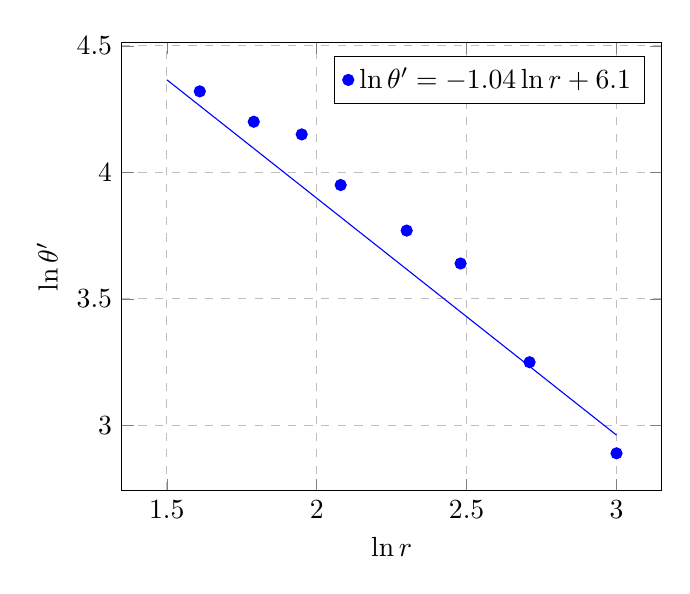
\begin{tikzpicture}
\begin{axis}[
    xlabel={$\ln r$},
    ylabel={$\ln \theta '$},
    ymajorgrids=true,
    xmajorgrids=true,
    grid style=dashed,
    legend pos=north east,
]

\addplot[
	only marks,
    color=blue,
    mark=*,
    ]
    coordinates {
	    (3,2.89)(2.71,3.25)(2.48,3.64)(2.3,3.77)(2.08,3.95)(1.95,4.15)(1.79,4.20)(1.61,4.32)
};
\addplot[color=blue, domain=1.5:3]{-0.936*x + 5.77};
\legend{$\ln \theta '=-1.04\ln r+6.1$}
    
\end{axis}
\end{tikzpicture}\\
Figure 2: Identifying $n$ by plotting $\ln r$ vs $\ln \theta '$
\end{center}

From \hyperref[fig:2]{figure 2}, we can see that $n=-1.04$, meaning $F\propto r^{-1.04}$. This is not what is predicted by Coulomb's law, so we must consider possible sources of error.

The error in each measurement of $\theta $ is $\Delta \theta =\theta_{\text{max}}-\theta _{\text{min}}$, and then the error in $\ln \theta $ to be $\Delta \theta /\theta $. For example, for $r=20$ cm, we have
\[
	\Delta \theta =20-14=6
.\]
\[
	\Delta \ln \theta = \frac{6}{18}=\frac{1}{3}
.\]
\hyperref[tab:4]{Table 4} depicts the errors in $\ln \theta $ for all $r$.
\begin{center}
	Table 4: Errors in $\ln \theta $\\\vspace*{5pt}
	\begin{tabular}{c|c}
		$r$ (cm)&$\Delta \ln \theta $ \\
		\hline
		20&0.33\\
		15&0.23\\
		12&0\\
		10&0\\
		8&0.23\\
		7&0\\
		6&0.05\\
		5&0
	\end{tabular}
\end{center}
To find the combined error, we take the square root of the sum of the squares of the errors:
\[
	\text{Error}=\sqrt{\sum_{i=1}^{8} \left( \Delta \ln (\theta_i) \right) ^2}
,\]
where $\Delta \ln (\theta _i)$ in this case means the error in the measurement of $\theta $ for the $i$th $r$ value. Plugging in, we have
\[
	\text{Error}=0.47
.\]
Since $n$ has a theoretical value of $-2$ and we experimentally identified a value of $-1.04$, we have an absolute difference of
\[
	\left| -2 +1.04\right| =0.96
.\]
Since our error is $0.47$, and $0.96>0.47$, our measurements do \textbf{not} agree with the theoretical values within error bounds.
\section{Conclusion}
Obviously, since Coulomb's law is an extremely well established scientific fact, we have no choice but to conclude that the error to align with theoretical values within the identified error is the fault of this experiment. The most likely reason our values are wrong is charge leakage. Charge can dissipate over time, especially so on a humid day. It was raining at the time of doing the lab, which means the humidity was likely quite higher. There was also some possible apparent evidence of charge leakage while peforming the experiment - sometimes, the ball would appear to \emph{almost} settle down to one side of the targetted position, but then would slowly move over to the target position. This suggests it was very likely our fault for waiting too long before making a measurement.

It's also possible the experimental apparatus contributed to the error. The balls were not exactly the same size, as the ball that was in motion appeared slightly smaller than the ball that was fixed to the sliding mechanism. This could have contributed greatly to the percieved error, but without knowledge of how the correction factor $B$ was determined, it's difficult to fully say what impact this had on the data.

While manipulating the experimental apparatus, the sliding part appeared to shift in position slightly relative to the rotational part. Slight variations in their relative position can impact data in multiple ways, such as making the apparent $r$ value inaccurate, or changing the angle the force forms with the rotational arm. Since we measured the torque, the latter would modify the results by a factor of $\cos \phi $, for an angle change of $\phi $.

Given so many unaccounted for possible sources of error, and such a large deviation from the theoretical value, it seems impossible that the results were free of error, and further trials in a more controlled environment may be needed to rectify the results of this paper.
\end{document}
